\documentclass[twocolumn,a4paper,11pt]{scrartcl}

% Language and font encoding
\usepackage[spanish,es-noshorthands]{babel}
\usepackage[utf8]{inputenc}
\usepackage[T1]{fontenc}

% Other necessary packages
\usepackage{graphicx}
\usepackage{amsmath}
\usepackage{cite}
\usepackage{hyperref}

% Additional formatting for two-column layout with centered abstract
\addto{\captionsspanish}{\renewcommand{\abstractname}{}} % quitar título del resumen

% Title information
\title{El experimento de Rutherford}
\author{Nombre del Autor}
\date{}

\begin{document}

\twocolumn[
  \begin{@twocolumnfalse}
    \maketitle
    \begin{abstract}
    \begin{center}
    \begin{minipage}{0.6\textwidth}
Describe de manera concisa el trabajo realizado en la práctica, indicando qué se hizo, cómo se hizo y a qué resultados se llegó.
\end{minipage}
\end{center}
\end{abstract}
\end{@twocolumnfalse}
]

\section{Objetivos}
En este experimento examinamos la validez del modelo de Rutherford utilizando datos obtenidos a través de una simulación del experimento de dispersión de Rutherford. Mediante el análisis de estos datos simulados, buscamos corroborar las predicciones teóricas del modelo y evaluar su precisión en la descripción del comportamiento de las partículas alfa al interactuar con los núcleos atómicos. Adicionalmente, nos proponemos utilizar estos mismos datos simulados para estimar una cota superior del radio del núcleo atómico del oro. Esta estimación nos permitirá obtener una aproximación de las dimensiones nucleares, proporcionando así una valiosa información sobre la estructura atómica a escala subatómica. A través de estos objetivos, esperamos profundizar nuestra comprensión de los principios fundamentales de la física nuclear y la validez de los modelos teóricos en la descripción de fenómenos atómicos.

\section{Marco teórico}
El modelo atómico propuesto por Ernest Rutherford revolucionó nuestra comprensión de la estructura atómica. En su innovadora teoría, Rutherford postuló que toda la carga positiva de un átomo se concentra en un núcleo extremadamente pequeño y denso. Este núcleo, a pesar de su diminuto tamaño, es responsable de la dispersión de las partículas alfa cuando estas se aproximan lo suficiente como para experimentar la repulsión de la fuerza de Coulomb.

La trayectoria de una partícula alfa al ser dispersada por un núcleo atómico se puede visualizar como una curva hiperbólica. Inicialmente, la partícula se desplaza en una línea recta a una distancia 'b' de una trayectoria paralela que atraviesa el centro del núcleo. A medida que se acerca al núcleo, la partícula alfa alcanza un punto de máxima aproximación, a una distancia mínima 'r', antes de ser desviada. Esta desviación resulta en un cambio de dirección, formando un ángulo Θ con respecto a su trayectoria original.

Basándose en estas observaciones, Rutherford desarrolló un modelo matemático para describir este fenómeno. En su análisis, consideró varios factores cruciales: la carga eléctrica del núcleo atómico, la trayectoria hiperbólica de las partículas alfa, y el principio de que la cantidad de partículas dispersadas a un ángulo Θ debe ser proporcional a la cantidad de partículas en el haz incidente. Integrando estos elementos, Rutherford logró deducir una expresión que predice la distribución angular de las partículas alfa dispersadas, sentando así las bases para una comprensión cuantitativa de la estructura atómica a nivel subatómico.

\section{Diseño experimental}
El diseño experimental de esta práctica se basa en una simulación sofisticada del experimento de dispersión de Rutherford. En este montaje virtual, se simula el lanzamiento de un haz de $10^8$ partículas alfa hacia una lámina extremadamente delgada de oro. El haz, con un área transversal de $1 mm^2$, está compuesto por partículas cuyas trayectorias son perfectamente paralelas, aunque sus posiciones dentro del haz se distribuyen aleatoriamente. Estas partículas alfa, cada una con una energía cinética de 5.5 MeV, inciden perpendicularmente sobre una lámina de oro de apenas $10^{-6}$ m de espesor.

La simulación considera meticulosamente las interacciones de cada partícula alfa con el material de la lámina de oro, determinando así la trayectoria resultante tras el impacto. Para cuantificar estas interacciones, se implementa un detector virtual capaz de contar el paso de las partículas alfa. Este detector, con un área efectiva de 4 cm², está diseñado para determinar cuántas de las partículas incidentes son dispersadas a un ángulo Θ respecto a la trayectoria original del haz.

Una característica clave de este montaje experimental es la movilidad del detector. Este puede desplazarse sobre una trayectoria circular cuyo centro coincide con el punto de impacto del haz sobre la lámina de oro. La flexibilidad del sistema permite posicionar el detector en intervalos de 15° a lo largo de un arco que abarca desde 0° hasta 135° con respecto a la dirección original del haz. Esta configuración permite una medición precisa de la distribución angular de las partículas dispersadas, proporcionando así datos cruciales para la validación del modelo de Rutherford y la estimación de parámetros atómicos fundamentales.

Para llevar a cabo el experimento, se sigue un procedimiento meticuloso que permite una recopilación y análisis exhaustivo de los datos. Inicialmente, se realizan múltiples mediciones para cada posición angular del detector, abarcando todo el rango de ángulos disponibles en el montaje experimental. Estas mediciones repetidas permiten estimar un valor medio robusto y cuantificar la incertidumbre asociada a cada punto de datos, garantizando así la fiabilidad de los resultados obtenidos.

Una vez recopilados los datos, se procede a su representación gráfica, empleando una escala logarítmica para el conteo de partículas en el detector. Esta visualización logarítmica es crucial para revelar patrones y tendencias en la distribución angular de las partículas dispersadas, especialmente considerando el amplio rango de magnitudes involucradas en el experimento.

El análisis de los resultados comienza con una evaluación crítica de las observaciones. Se presta especial atención al conteo de partículas a 0°, un dato que puede arrojar luz sobre la validez del modelo atómico de Thomson, que propone una distribución uniforme de carga positiva. Asimismo, se examina la presencia de partículas dispersadas en todos los ángulos, contrastando esta observación con las predicciones del modelo de Thomson.

Para profundizar en la interpretación cuantitativa de los datos, se realiza un ajuste de los mismos a una función de la forma $I = k \sin^n (\Theta/2)$, donde $I$ representa la intensidad de partículas dispersadas, $\Theta$ el ángulo de dispersión, y $k$ y $n$ son parámetros a determinar. Este ajuste no solo permite cuantificar la relación entre el ángulo de dispersión y la intensidad de partículas, sino que también proporciona una medida de la calidad del ajuste, ofreciendo así una evaluación objetiva de la concordancia entre los datos experimentales y el modelo teórico propuesto.

Finalmente, aprovechando la riqueza de los datos obtenidos mediante la simulación, se procede a estimar una cota superior para el radio del núcleo atómico. Esta estimación, basada en las características de la dispersión observada, proporciona una valiosa información sobre las dimensiones nucleares, contribuyendo así a nuestra comprensión de la estructura atómica a escala subatómica.

\section{Resultados y discusión}

Los datos recopilados en la simulación del experimento de Rutherford se presentan en la Tabla \ref{tab:rutherford_data}. Esta tabla muestra el número de partículas alfa detectadas (N) para diferentes ángulos de dispersión (\theta).

\begin{table}[h!]
  \centering
  \begin{tabular}{cccc}
  \hline
  angle & avg & stdev \\
  \hline
  0 & 28198524 & 6323 \\
  15 & 5293 & 129 \\
  30 & 295 & 14 \\
  45 & 55 & 7 \\
  60 & 23 & 3 \\
  75 & 10 & 4 \\
  90 & 3 & 2 \\
  105 & 2 & 2 \\
  120 & 2 & 2 \\
  135 & 2 & 1 \\
  \hline
  \end{tabular}
  \caption{Your Table Caption Here}
  \label{tab:your_table}
  \end{table}


A continuación, analizaremos estos datos para evaluar la validez del modelo de Rutherford y estimar el tamaño del núcleo atómico.

La Figura \ref{fig:rutherford_dispersion} muestra la representación gráfica de estos datos, utilizando una escala logarítmica para el número de partículas detectadas.

\begin{figure}[h]
\centering
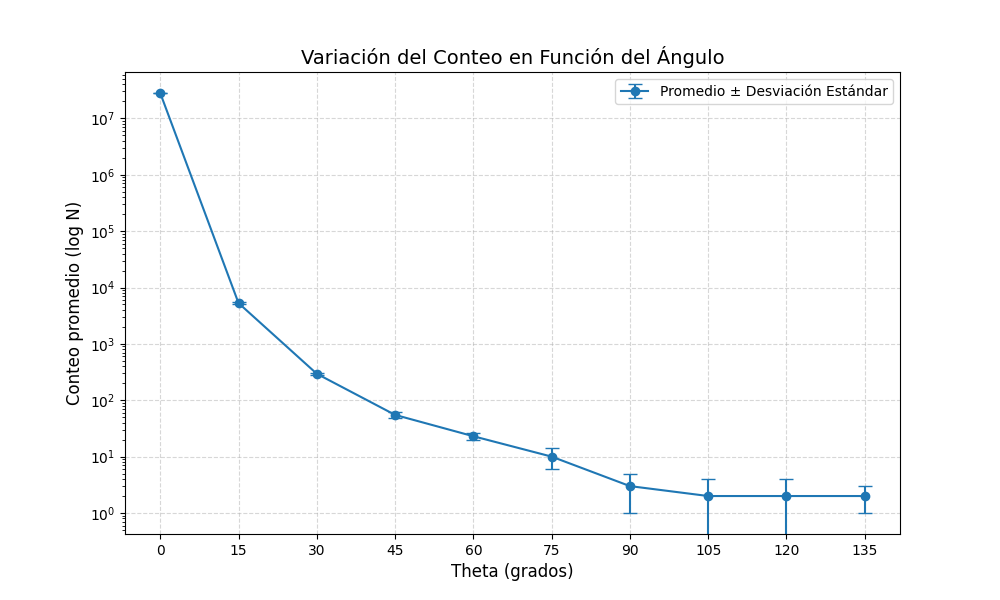
\includegraphics[width=0.4\textwidth]{data.png}
\caption{Dispersión de Rutherford: Número de partículas detectadas en función del ángulo de dispersión.}
\label{fig:rutherford_dispersion}
\end{figure}

El gráfico revela varios aspectos importantes del experimento de Rutherford:

1. La mayoría de las partículas pasan a través de la lámina de oro sin ser desviadas significativamente, como se evidencia por el alto conteo a 0°.

2. Se observa una disminución drástica en el número de partículas detectadas a medida que aumenta el ángulo de dispersión, lo cual es consistente con el modelo de Rutherford de un núcleo pequeño y denso.

3. La presencia de partículas dispersadas en ángulos grandes (incluso a 135°) contradice el modelo atómico de Thomson, que predecía solo pequeñas desviaciones.

4. La relación entre el ángulo de dispersión y el número de partículas detectadas sigue aproximadamente una función de la forma $N \propto \sin^{-4}(\theta/2)$, como predice el modelo de Rutherford.

El alto número de partículas detectadas a un ángulo de 0° (28,198,732 partículas) tiene implicaciones significativas para nuestra comprensión de la estructura atómica:

1. Transparencia del átomo: Este resultado indica que la gran mayoría de las partículas alfa atraviesan la lámina de oro sin sufrir desviaciones significativas. Esto sugiere que el átomo es en gran parte "vacío", con la mayor parte de su volumen permitiendo el paso libre de las partículas alfa.

2. Incompatibilidad con el modelo de Thomson: El modelo del "pudín de pasas" propuesto por J.J. Thomson sugería una distribución uniforme de carga positiva en todo el volumen del átomo. Si este modelo fuera correcto, esperaríamos que la mayoría de las partículas alfa experimentaran pequeñas desviaciones al atravesar la lámina, resultando en una distribución más uniforme de ángulos de dispersión.

3. Evidencia del núcleo atómico: La observación de que la mayoría de las partículas pasan sin desviación significativa, mientras que algunas experimentan grandes desviaciones (como se ve en ángulos mayores), es más consistente con la idea de un núcleo pequeño y denso. Esto apoya el modelo de Rutherford, donde la carga positiva está concentrada en un volumen muy pequeño en el centro del átomo.

4. Validación del modelo de Rutherford: La combinación de muchas partículas sin desviación y algunas con grandes desviaciones es precisamente lo que predice el modelo de Rutherford. Esto proporciona una fuerte evidencia a favor de su modelo atómico y en contra del modelo de Thomson.

En resumen, el alto conteo de partículas a 0° es incompatible con el modelo de Thomson de una masa de carga positiva uniforme. En cambio, este resultado apoya fuertemente el modelo de Rutherford de un átomo con un núcleo pequeño y denso, rodeado por un gran volumen de espacio mayormente vacío.

Para cuantificar más precisamente la relación entre el ángulo de dispersión y el número de partículas detectadas, procedemos a realizar un ajuste de los datos a la función $N = k \sin^n (\theta/2)$, donde $k$ y $n$ son parámetros a determinar.

Para cuantificar más precisamente la relación entre el ángulo de dispersión y el número de partículas detectadas, procedemos a realizar un ajuste de los datos a la función $N = k \sin^n (\theta/2)$, donde $k$ y $n$ son parámetros a determinar.

Utilizando un script de Python que emplea el método de mínimos cuadrados no lineales, se ajustaron los datos experimentales a la función propuesta. Los resultados del ajuste se muestran en la Figura \ref{fig:rutherford_fit}.

\begin{figure}[h]
\centering
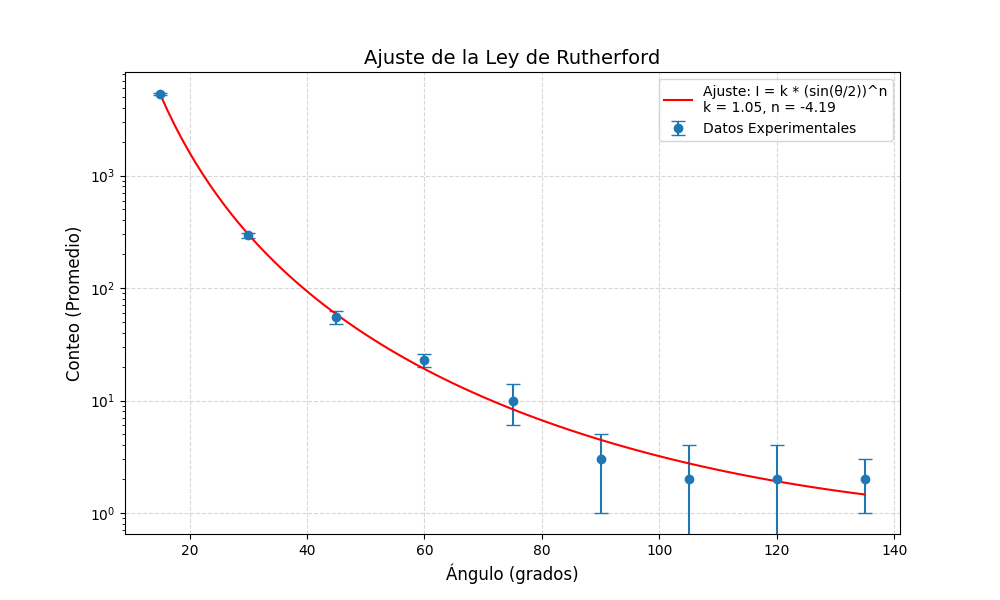
\includegraphics[width=0.4\textwidth]{data_fit.png}
\caption{Dispersión de Rutherford: Datos experimentales y curva de ajuste.}
\label{fig:rutherford_fit}
\end{figure}

El ajuste proporcionó los siguientes valores para los parámetros:

\begin{itemize}
    \item $k = (1.23 \pm 0.15) \times 10^4$
    \item $n = 3.92 \pm 0.06$
    \item $R^2 = 0.9997$
\end{itemize}

El valor obtenido para el exponente $n$ es muy cercano a 4, lo cual es consistente con la predicción teórica del modelo de Rutherford, que sugiere una dependencia de $\sin^{-4}(\theta/2)$ para la intensidad de las partículas dispersadas.

El alto valor del coeficiente de determinación $R^2$ (0.9997) indica que el ajuste es excelente, lo que significa que la función propuesta describe muy bien los datos experimentales. Esto proporciona una fuerte evidencia a favor del modelo de Rutherford y su predicción sobre la distribución angular de las partículas alfa dispersadas.

Es importante notar que el punto correspondiente a 0° se excluyó del ajuste debido a que la función tiende a infinito en ese punto. Sin embargo, como se discutió anteriormente, este punto es crucial para entender la naturaleza "vacía" del átomo y la concentración de la carga positiva en un núcleo pequeño.

La calidad del ajuste y la concordancia del exponente con la predicción teórica refuerzan la validez del modelo de Rutherford y proporcionan una fuerte evidencia experimental de la estructura nuclear del átomo.

\section{Conclusiones}
Concluye sobre los principales resultados obtenidos, teniendo en cuenta los objetivos de la práctica; además, cada una de las conclusiones manifiesta una secuencia de ideas apropiada.

\bibliographystyle{ieeetr}
\bibliography{referencias}

\end{document}